% tirlnx01 - Materiaal om het keuzevak Linux te geven 
% op de Hogeschool Rotterdam.
% Copyright (C) 2010 - 2011  Paul Sohier, Kevin van der Vlist
%
% This program is free software: you can redistribute it and/or modify
% it under the terms of the GNU General Public License as published by
% the Free Software Foundation, either version 3 of the License, or
% (at your option) any later version.
%
% This program is distributed in the hope that it will be useful,
% but WITHOUT ANY WARRANTY; without even the implied warranty of
% MERCHANTABILITY or FITNESS FOR A PARTICULAR PURPOSE.  See the
% GNU General Public License for more details.
%
% You should have received a copy of the GNU General Public License
% along with this program.  If not, see <http://www.gnu.org/licenses/>.
%
% Kevin van der Vlist - kevin@kevinvandervlist.nl
% Paul Sohier - paul@paulsohier.nl

\chapter{Editors}
Op een \emph{Linux} systeem zijn er verschillende \emph{editors}, ofwel tekstverwerkers beschikbaar. De verschillende \emph{editors} hebben allemaal een eigen doelgroep. Zo zijn er \emph{editors} die zich richten op beginnende gebruikers, zoals \texttt{pico}\index{pico}, maar zijn er ook erg geavanceerde programma's als \texttt{emacs}\index{emacs} of \texttt{vim}\index{vim}. 

Een programma als \texttt{pico}\index{pico} is gemakkelijk in het gebruik, er is weinig voorkennis vereist om ermee te werken. Bij \emph{editors} als \texttt{emacs}\index{emacs} of \texttt{vim}\index{vim} is dit het tegenovergestelde. Dit betekent echter wel dat, eenmaal hieraan gewend, dat deze ontzettend snel werken. Verder hebben ze als voordeel dat ze gebruikers beschermen voor dingen als \emph{RSI}, omdat muis gebruik wordt vermeden. 

Vanuit historisch oogpunt is er altijd een laconieke vete geweest tussen twee kampen; \texttt{emacs}\index{emacs} en \texttt{vim}\index{vim}. Dit wordt de \emph{editor wars} genoemd. Er is geen enkele manier om sneller een discussie aan te wakkeren dan te melden dat een van de twee ``veel beter'' is dan de ander.

\section{Pico}
\texttt{pico}\index{pico} is een simpel scherm geori\"{e}nteerde tekst editor. Om de \emph{teksteditor} \texttt{pico}\index{pico} te starten volstaat het om het volgende uit te voeren: 
\begin{lstlisting}
kevin@slackbak:~$ pico document.txt
\end{lstlisting}%$
Het bestand \emph{document.txt} zal nu worden geopend. Mocht het bestand niet bestaan dan zal \texttt{pico}\index{pico} nog steeds opstarten en beginnen in een nieuw bestand met de naam \emph{document.txt}.

\texttt{nano} is een uitgebreide/verbetererde versie van \texttt{pico}.\index{nano} Bij veel distributies zal standaard zowel \emph{pico} als \emph{nano} ge\"{i}nstalleerd zijn. De interface en toetsencombinaties in \emph{nano} werken hetzelfde als die in \emph{pico}.

\subsection{Bediening}
Wanneer \texttt{pico}\index{pico} start zal er onderin het scherm het een en ander aan mogelijkheden staan. Deze opties zijn te gebruiken met de toetscombinnatie die ervoor staat. Het dakje \emph{\^{}} staat voor \emph{ctrl}. De toetsencombinatie \emph{\^{}X} betekent dus \emph{ctrl-X}. De letters zijn niet hoofdlettergevoelig. 

Een ander handigheidje binnen \texttt{pico}\index{pico} is het gebruik van de \emph{kill buffer}. Wanneer de combinatie \emph{\^{}K} wordt gebruikt, zal de huidige regel worden geknipt. Als hij weer moet worden geplakt kan dit gedaan worden met \emph{\^{}K}. 

Zodra er in de huidige \emph{buffer} een wijziging heeft plaatsgevonden zal de tekst \emph{modified} onder in beeld komen. Wanneer \texttt{pico}\index{pico} nu afgesloten wordt zonder het bestand op te slaan, zal deze uit zichzelf een waarschuwing laten zien. Er kan dan alsnog worden gekozen om het bestand op te slaan. 

\section{VI(M)}
\emph{The number of the beast: VI VI VI}\\\\
De bekendste \emph{UNIX} editor is zonder twijfel \texttt{vi}\index{vi}. Deze editor is op elk \emph{UNIX} systeem standaard ge\"{e}nstalleerd en door velen gehaat. \texttt{vim}\index{vim} is een verbeterde versie van \texttt{vi}\index{vi} en werkt vele malen gemakkelijker.

\texttt{vim}\index{vim} is in hoge mate configureerbaar en heeft vrijwel eindeloze mogelijkheden. De bijlage \ref{app.vim} beschrijft enkele configuratie mogelijkheden van \texttt{vim}\index{vim}. 
\begin{figure}[H]
  \begin{center}
    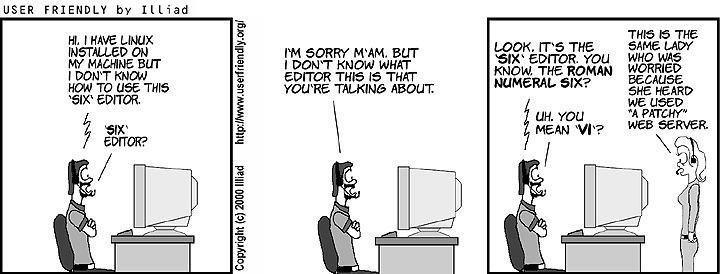
\includegraphics[scale=0.5]{images/uf001688}
  \end{center}
  \caption{Van:userfriend.org}
  \label{fig:setup}
\end{figure}

\section{Emacs}
Omdat er ook mensen waren die met een \emph{handige} \emph{editor} wilden werken, is er ook \'{e}\'{e}n onstaan met de naam \texttt{emacs}\index{index}. Deze \emph{editor} is nog modulairder dan \texttt{vim}\index{vim} en is volgens velen ook handiger in gebruik, al is dit een gegarandeerd discussiepunt. In bijlage \ref{app.emacs} is een kleine inleiding tot het gebruik van \texttt{emacs}\index{emacs} te vinden. 

\begin{figure}[H]
  \begin{center}
    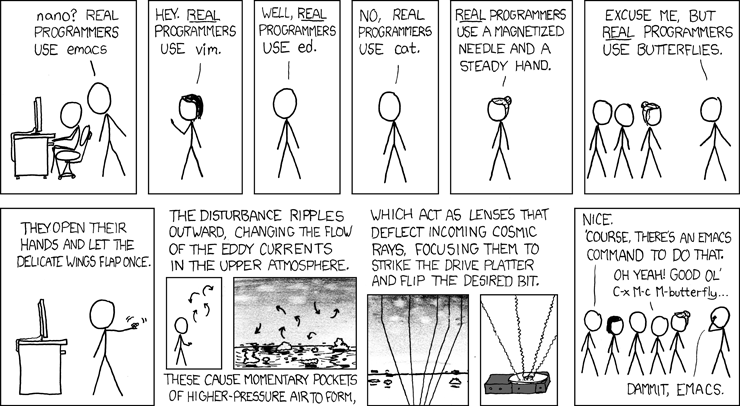
\includegraphics[scale=0.5]{images/real_programmers}
  \end{center}
  \caption{Van:xkcd.org}
  \label{fig:XKCD_emacs_butterfly}
\end{figure}
